%! TEX root = ../root/raiz.tex
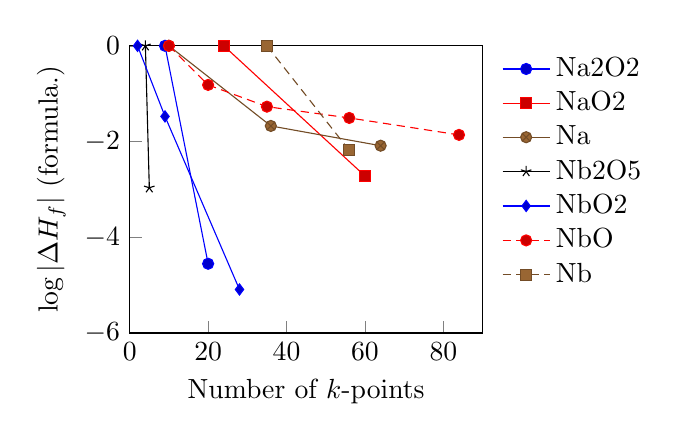
\begin{tikzpicture}
\begin{axis}[
    width=0.5\linewidth,
    legend pos={outer north east},
    legend style={draw=none},
    legend cell align=left,
    tick align=inside,
    tick pos=left,
    minor tick num=0,
    xlabel={Number of $k$-points},
    xmin=0, xmax=90,
    ylabel={$\log|\Delta H_f|$ (\si{\electronvolt\per formula}.)},
    ymin=-6, ymax=0
]
\addplot table {%
9  0
20 -4.553
};
\addplot table {%
24	0
60	-2.719
};
\addplot table {%
10	0
36	-1.674
64	-2.087
};
\addplot table {%
4	0
5	-2.966
};
\addplot table {%
2	0
9	-1.475
28	-5.091
};
\addplot table {%
10	0
20	-0.817
35	-1.271
56	-1.507
84	-1.861
};
\addplot table {%
35	0
56	-2.184
};
\legend{\ce{Na2O2},\ce{NaO2},\ce{Na},\ce{Nb2O5},\ce{NbO2},\ce{NbO},\ce{Nb}}
\end{axis}
\end{tikzpicture}
